\begin{problem}\textbf{Cycle in Graph}

    Given a graph $g$ of $n$ verticies and $m$ edges. Find any cycle in the given graph and print its verticies.
\end{problem}


\begin{solution}

    The idea is to implement dfs with \textbf{two colors}:

    1. \textit{Color 1} denotes that this vertex was visited but yet not left by the dfs.

    2. \textit{Color 2} denotes that this vertex was left by the dfs.

    The cycle is a situation in the dfs algorithm when it encounters any vertex that has a color $1$. Once such vertex is found the graph has a cycle.

    In order to print its verticies we need to keep track of the visited but yet not left verticies (i.e. verticies of color 1). We can implement it by inserting a currently considered vertex inside an vector and remove it from the vector once all its neighbouring verticies are traversed. Once the cycle is found ending at the vertex $v$ of color $1$, we will go through the elements of this tracking vector until and print its elements until $v$ is found.

    \begin{lstlisting}[language=C++]
    bool dfs(int v, vector<int>& trace) {
        if (marked[v] == 2) return false;
        if (marked[v] == 1) {
            // found cycle
            std::cout << v << " ";
            while(trace.back() != v) {
                std::cout << trace.back() << " ";
                trace.pop_back();
            }
            return true;
        }

        marked[v] = 1;
        trace.push_back(v);

        // traverse neighbouring verticies
        bool found = false;
        for (int u : graph[v]) {
            found = dfs(u);
            if (found) break;
        }

        trace.pop_back();
        return found;
    }
    \end{lstlisting}

\end{solution}


\begin{problem}\textbf{2285. Maximum Total Importance of Roads}

    You are given an integer $n$ denoting the number of cities in a country. The cities are numbered from $0$ to $n-1$. You are given the set of roads $r$ between the cities $a_i \to b_i$.

    You need to assign integer values from $1$ to $n$ to all the cities, where each value can only be used \textbf{once}.

    \underline{Definition}: The \textbf{importance} of a road is the sum of the values of the two cities it connects.

    Return the \textbf{maximum total importance} of all roads possible after assigning the values optimally.\\

    \underline{Note}: you may solve this problem on LeetCode, \href{https://leetcode.com/problems/maximum-total-importance-of-roads/description/}{2285. Maximum Total Importance of Roads}.

    \begin{center}
        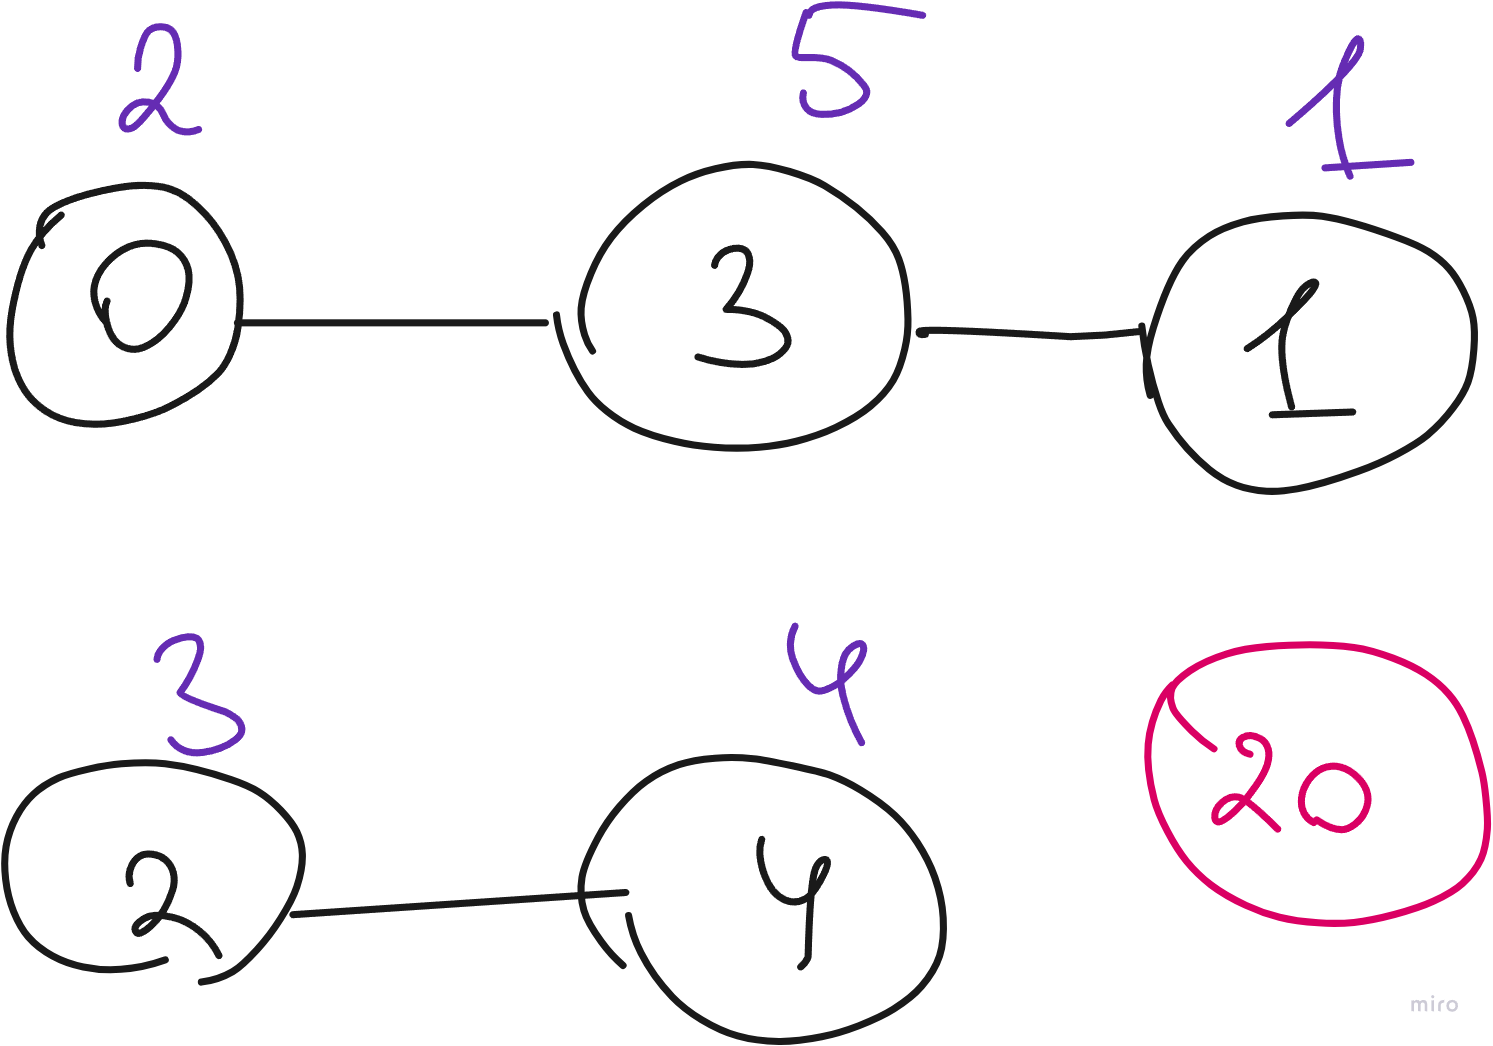
\includegraphics[scale=0.11]{./assets/14-graphs-and-basic-dfs/1.png}

        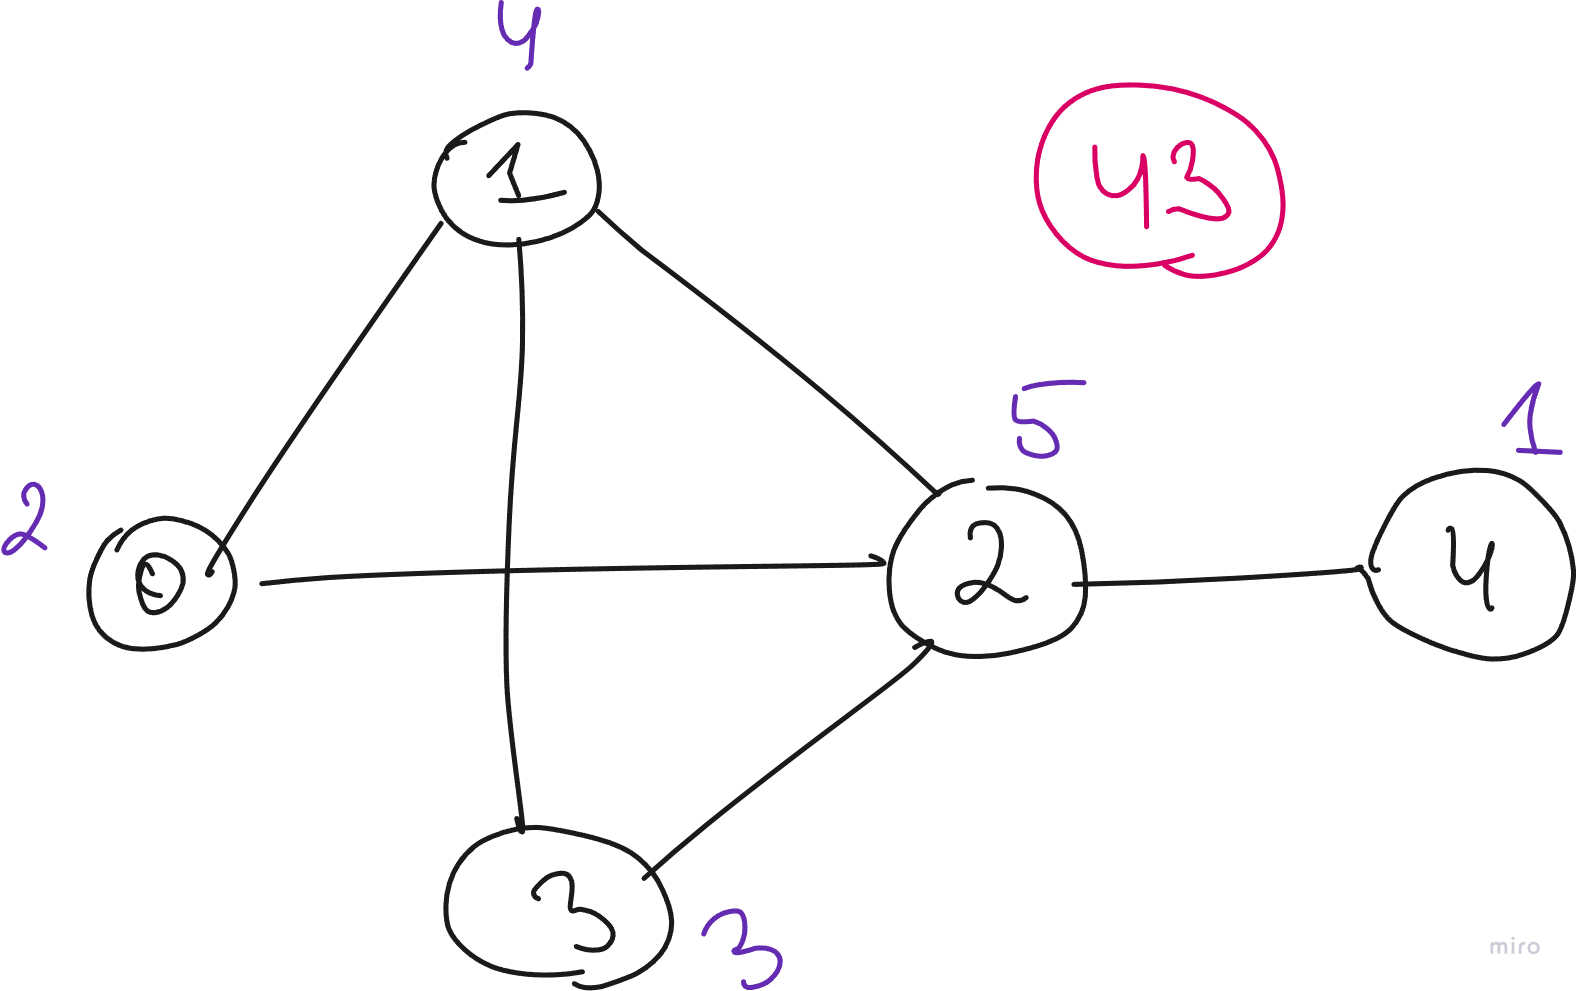
\includegraphics[scale=0.11]{./assets/14-graphs-and-basic-dfs/2.png}
    \end{center}

\end{problem}


\begin{solution}

    Let's consider a single vertex $v$ with assigned value $i_v$ and its contribution to the result: $\deg{v} \cdot i_v$.

    The total importance is calculated as follows: $S := \sum_{v \in V} i_v \cdot \deg{v} \to \max$. Notice that $S$ takes its maximum when we assign greater values $i_v$ to verticies with greater $\deg$. Thus, let's sort the verticies according their degrees $\deg{v}$ in the ascending order and assign values from $1$ to $n$ in such order:

    \begin{lstlisting}[language=C++]
        int maximumImportance(vector<pair<int>>& roads) {
            vector<int> deg(n);
            for (auto [v, u] : roads) {
                ++deg[v];
                ++deg[u];
            }

            vector<int> verticies(n);
            for (int i = 0; i < n; ++i) {
                verticies[i] = i;
            }

            std::sort(std::begin(verticies), std::end(verticies), [&](int v, int u) {
                return deg[v] < deg[u];
            });

            int S = 0;
            for (int value = 1; value <= n; ++value) {
                int v = verticies[value - 1];
                S += value * deg[v];
            }

            return S;
        }
    \end{lstlisting}

\end{solution}